\documentclass{article}

\usepackage{listings}
\usepackage{xcolor}
\usepackage{courier}
\usepackage{graphicx}
%\graphicspath{{./figures/}}
\usepackage{float}
\usepackage[hidelinks]{hyperref}
\usepackage{caption}
\captionsetup[table]{name=جدول}
\usepackage{indentfirst}
\usepackage{multicol}
\usepackage{imakeidx}
%\usepackage{float}

\usepackage{xepersian}
\settextfont{HMXZar}
\setdigitfont{Times New Roman}

\definecolor{lightgray}{gray}{0.95}

\lstset{
%basicstyle=\ttfamily,
backgroundcolor=\color{lightgray},
numbers=left,
tabsize=4,
frame=tblr,
breaklines=true, 
captiondirection=RTL, 
language=C++, 
belowcaptionskip=1\baselineskip,
%frame=none,
basicstyle=\footnotesize\ttfamily,
keywordstyle=\bfseries\color{green!40!black},
commentstyle=\itshape\color{purple!40!black},
identifierstyle=\color{blue},
%backgroundcolor=\color{gray!10!white},
} % adapted from https://nasa.github.io/nasa-latex-docs/html/examples/listing.html
\renewcommand\lstlistingname{\rl{کد}}

\def\codename#1{\lr{\lstinline{#1}}}
\def\itname#1{\lr{\textit{#1}}}
\def\streamop{\codename{<<}}
\def\experimental{\textcolor{red}{(آزمایشی)}}
\def\deprecated{\textcolor{blue}{(توصیه نمی‌شود)}}

\def\idxlib#1{\index{#1, library}}
\def\idxclass#1{\index{#1, class}}
\def\idxfunc#1{\index{#1, function}}
\def\idxtype#1{\index{#1, datatype}}
\def\idxvar#1{\index{#1, variable}}

\title{راهنمای برنامه‌نویسی با استفاده از \lr{uv2cnf}}
\date{تیر ۱۴۰۰}
\author{محمد (رها) مرادی شهمیری\\\lr{raham9619@gmail.com}}

\indexsetup{level=\section}
\makeindex[title={\rl{فهرست الفبایی}},intoc]

\begin{document}
\pagenumbering{gobble}
\maketitle
\newpage
\rl{\tableofcontents}
\newpage

\pagenumbering{arabic}

\section{مقدمه}

نرم‌افزار \lr{uv2cnf} برای تبدیل توصیف سطح گیت مدارات ترکیبی به معادلات cnf مناسب برای دیباگ کاربرد دارد. اصول کارکرد این برنامه در راهنمای استفاده [cite] بررسی شده است. در اینجا به کتابخانه‌های تشکیل‌دهنده‌ی آن، طرز استفاده از آن‌ها در این برنامه و نحوه‌ی توسعه‌ی برنامه‌های دیگر بر مبنای آن‌ها پرداخته می‌شود. در ادامه‌ی قسمت اول ساختار کلی برنامه و جایگاه هر جزء و نحوه‌ی ارتباط آن‌ها با هم بررسی می‌شود. در هر کدام از قسمت‌های بعدی یکی از اجزای اصلی بررسی می‌شود. 

یک \underline{محدودیت} کتابخانه‌های نوشته‌شده این است که تنها از پورت‌های تک‌بیتی پشتیبانی می‌کنند (آرایه تعریف نشده است). 

\section{نرم‌افزار \lr{uv2cnf}}

کد اصلی برنامه در فایل \textit{main.cpp} قرار دارد و صرف نظر از مواردی که برای گزارش‌دهی و بررسی صحت پارامترها در نظر گرفته شده، بدین ترتیب کار می‌کند:‌ 
\begin{enumerate}
\item
کتابخانه‌ی ورودی (با فرمت \textit{cnflib}) را می‌خواند. 
\item
فایل وریلاگ داده‌شده را می‌خواند. 
\item
به ازای هر ماژول در فایل ورودی
\begin{enumerate}
\item
ماژول را با استفاده از کتابخانه‌ی داده‌شده به فرمت cnf express تبدیل می‌کند. 
\item
بر اساس متغیرهای ماژول یک جدول از متغیرها می‌سازد.
\item
در صورت وجود، فایل راه حل را خوانده و جمله‌های مربوط به آن را به تابع اضافه می‌کند.
\item
در صورت وجود، فایل محدودیت تعداد را خوانده و جمله‌های مربوط به آن را به ورودی اضافه می‌کند. 
\item
با استفاده از جدول متغیرهای تولیدشده، نمایش cnf express را به cnf تبدیل می‌کند. 
\item
بر اساس پیشوند مسیر داده‌شده، نام فایل cnf خروجی را تولید کرده و تابع را در آن می‌نویسد. 
\item
بر اساس پیشوند مسیر داده‌شده، نام فایل map خروجی را تولید کرده و نگاشت متغیرهای متناظر با جدول متغیرهای ماژول را در آن می‌نویسد. 
\end{enumerate}
\end{enumerate}

در بقیه‌ی این راهنما جزئیات کارکرد هرکدام از کتابخانه‌های به‌کاررفته بررسی می‌شود. برای توضیح بیشتر در مورد نمایش cnf و cnf express به قسمت ref{section:libcnf} همین راهنما و برای توضیح در مورد سایر فرمت‌های به‌کاررفته ({libcnf}، {sol} و {card})‌به \textit{دستورالعمل راهنما} مراجعه شود. 

\section{\lr{libcnf}}\label{section:libcnf}\idxlib{libcnf}

این کتابخانه امکان خواندن، نوشتن و پردازش توابع منطقی با نمایش cnf را فراهم می‌کند. با استفاده از کلاس‌های این کتابخانه توابع را در دو فرم cnf استاندارد و با نام متغیرها نمایش داد. به عنوان مثال، اگر متغیر‌های {W}، {A} و {B} به ترتیب به شماره‌های ۱، ۲ و ۳ نگاشته شده باشند، نمایش 

\begin{flushleft}\lr{$(W + A)(W + B)(W' + A' + B')$}\end{flushleft}

با نمایش 

\begin{flushleft}\lr{$1\;2\;0$\\
$1 \; 3 \; 0$\\
$-1\;-2\;-3\;0$}\end{flushleft}

معادل است. برای نوشتن معادله ابتدا کد توصیف سخت‌افزار بر حسب متغیرها به شکل cnf نوشته شده، سپس با تخصیص شماره‌های یکتا به متغیرها معادله به فرم cnf استاندارد مناسب برای solver درمی‌آید. 

\subsection{کلاس \lr{\_\_cnf\_temp\_class}}\idxclass{\_\_cnf\_temp\_class}

این کلاس به عنوان پایه برای بیشتر کلاس‌های libcnf تعریف شده و تعریف آن مطابق کد \ref{lst:cnftempclass} است. 

\lstset{caption={تعریف کلاس \_\_cnf\_temp\_class},label=lst:cnftempclass}
\LTR{
\begin{lstlisting}
template <typename T> class __cnf_temp_class
{
protected:
    std::vector<T> things;
public:
    void __CTOR () {}
    template <typename...X>
    void __CTOR (T item, X...args);
    __cnf_temp_class() {}
    template <typename...X>
    __cnf_temp_class (T item, X...args);
    T& operator [] (int num);
    int size();
    void resize (unsigned size);
    void add (T item);
};
\end{lstlisting}}\RTL{}
\idxfunc{\_\_cnf\_temp\_class.size}
\idxfunc{\_\_cnf\_temp\_class.resize}
\idxfunc{\_\_cnf\_temp\_class.add}
\idxvar{\_\_cnf\_temp\_class.things}
وکتور \lr{\lstinline{things}} دیتای کلاس را نگه داشته و توابع {\lr{\lstinline{size}}}، \lr{\lstinline{resize}} و \lr{\lstinline{add}} به ترتیب برای گرفتن اندازه، تنظیم اندازه و افزودن عنصر جدید به وکتور به کار می‌روند. یک خاصیت مهم این کلاس constructor آن است که با استفاده از قابلیت variadic template زبان \lr{C++} امکان مقداردهی اولیه با تعداد متغیری از آرگومان‌ها را فراهم می‌کند. از این قابلیت برای تعریف جمله‌ها و تابع‌های منطقی پیش‌فرض استفاده می‌شود که در قسمت‌های مربوط، مثال‌هایی از آن بررسی می‌شود. 

\subsection{کلاس \lr{assignment}}

این کلاس برای نگه‌داری یک پاسخ معادله در قالب نگاشتی از متغیرها به مقادیر منطقی به کار می‌رود و کاربرد اصلی آن در تابع \lr{\lstinline{eval}} از کلاس \lr{\lstinline{clause}} است که بررسی خواهد شد. تعریف این کلاس مطابق کد \ref{lst:assignment} است. 

\lstset{caption={تعریف کلاس assignment},label=lst:assignment}
\LTR{
\begin{lstlisting}
class assignment : public __cnf_temp_class<unsigned short>
{using __cnf_temp_class::__cnf_temp_class; };
\end{lstlisting}}\RTL{}

\subsection{کلاس \lr{clause}}\idxclass{clause}

این کلاس برای نگه‌داری یک جمله به کار می‌رود که شامل \textit{OR} منطقی تعدادی متغیر و نقیض متغیر است. تعریف این کلاس مطابق کد \ref{lst:clause} است. 

\lstset{caption={تعریف کلاس clause},label=lst:clause}
\LTR{
\begin{lstlisting}
class clause : public __cnf_temp_class<int32_t>
{
    using __cnf_temp_class::__cnf_temp_class;
public: 
    bool eval (assignment& value);
    void add (int v);
};
\end{lstlisting}}\RTL{}
\idxfunc{clause.eval}
\idxfunc{clause.add}
تابع \codename{eval} برای ارزیابی یک جمله بر حسب یک مقداردهی معین از متغیرها به کار می‌رود. وظیفه‌ی تابع \codename{add} افزودن یک عنصر جدید به جمله است. برای روشن‌شدن کاربرد این کلاس،  مثالی از آن در کد \ref{lst:clauseex} آمده است. 

\lstset{caption={مثالی از کاربرد کلاس clause},label=lst:clauseex}
\LTR{
\begin{lstlisting}
clause newclause(1, -2, 3);
		// equivalent to `1 -2 3 0` in cnf representation
std::cout << newclause.eval(assignment(1, 0, 1));	// prints `1`
std::cout << newclause.eval(assignment(1, 1, 1));	// prints `0`
\end{lstlisting}}\RTL{}

\subsection{کلاس \lr{cnf}}\idxclass{cnf}

این کلاس برای نگه‌داری توابع منطقی با نمایش cnf به کار می‌رود و تعریف آن مطابق کد \ref{lst:cnf} است. 

\lstset{caption={تعریف کلاس cnf},label=lst:cnf}
\LTR{
\begin{lstlisting}
class cnf : public __cnf_temp_class<clause>
{
    using __cnf_temp_class::__cnf_temp_class;
public:
    bool eval (assignment& value);
    int varnum();
    void add (clause cc);
};
\end{lstlisting}}\RTL{}
\idxfunc{cnf.eval}
\idxfunc{cnf.varnum}
\idxfunc{cnf.add}
توابع \codename{eval} و \codename{add} مشابه معادل‌هایشان در کلاس \codename{clause} رفتار می‌کنند. تابع \codename{eval} توابع متناظر مربوط به تک‌تک جمله‌ها را فراخوانده و خروجی‌هایشان را با هم \textit{AND} می‌کند. تابع \codename{varnum} متغیرهای موجود در تابع را می‌شمارد. نحوه‌ی نمایش یک تابع منطقی با استفاده از این کلاس در کد \ref{lst:cnfex} نمایش داده شده است. 

\lstset{caption={مثالی از کاربرد کلاس cnf},label=lst:cnfex}
\LTR{
\begin{lstlisting}
cnf function(clause(1, 2), clause(2, 3), clause(1, 3), clause (-1, -2, -3));
// equivalent to the following cnf representation: 
// p cnf 3 4
// 1 2 0
// 2 3 0
// 1 3 0
// -1 -2 -3 0
\end{lstlisting}}\RTL{}

برای کلاس \codename{cnf} عملگر \streamop تعریف شده که امکان تولید خروجی فرمت cnf از متحوای کلاس را فراهم کرده و برای ذخیره‌ی خروجی در قالب فایل cnf به کار می‌رود. 

\subsection{کلاس \lr{clause\_express}}\idxclass{clause\_express}

این کلاس جمله‌های با فرمت cnf را بر حسب نام متغیرها ذخیره می‌کند. در نمایش به‌کاررفته در این کلاس، نقیض (\textit{NOT}) متغیر $x$ به صورت \lr{$x'$} ذخیره می‌شود. همچنین برای نمایش جمله به شکل خوانا عملگر \streamop برای آن تعریف شده است. تعریف این کلاس در کد \ref{lst:clauseexpress} و مثالی از کاربرد آن در کد \ref{lst:clauseexpressex} آمده است. 

\lstset{caption={تعریف کلاس clause\_express},label=lst:clauseexpress}
\LTR{
\begin{lstlisting}
class clause_express : public __cnf_temp_class<std::string>
{
    using __cnf_temp_class::__cnf_temp_class;
};
\end{lstlisting}}\RTL{}

\lstset{caption={مثالی از کاربرد کلاس clause\_express},label=lst:clauseexpressex}
\LTR{
\begin{lstlisting}
clause_express testclause("a", "b'", "c");
std::cout << testclause << std::endl;
// Prints `a+b'+c`
\end{lstlisting}}\RTL{}

\subsection{کلاس \lr{cnf\_express}}\label{section:cnfexpress}\idxclass{cnf\_express}

این کلاس امکان نگه‌داری نمایش cnf توابع منطقی به شکل خوانا را فراهم می‌کند. رابطه‌ی \codename{cnf\_express} با \codename{clause\_express} مانند رابطه‌ی \codename{clause} با \codename{cnf} است. برای این کلاس عملگرهای \streamop و \lr{\&=} تعریف شده‌اند که به ترتیب امکان نمایش تابع و \textit{AND} کردن دو تابع مختلف با هم را فراهم می‌کنند. تعریف این کلاس در کد \ref{lst:cnfexpress} مشاهده می‌شود. 

\lstset{caption={تعریف کلاس cnf\_express},label=lst:cnfexpress}
\LTR{
\begin{lstlisting}
class cnf_express : public __cnf_temp_class<clause_express>
{
    using __cnf_temp_class::__cnf_temp_class;
public: 
    void operator &= (cnf_express param);
};
\end{lstlisting}}\RTL{}

کلاس \codename{cnf\_express} دو کاربرد اساسی در تبدیل کد وریلاگ به نمایش cnf دارد. نخست این که به دلیل استفاده از نام اصلی متغیرها، به عنوان واسطه میان توصیف سخت‌افزار و نمایش ریاضی عمل می‌کند. دوم این که در نمایش cnf به دلیل استفاده از اعداد برای نمایش متغیرها امکان انجام عملیات منطقی روی آن‌ها به صورت مستقیم وجود ندارد، مگر این که از پیش نگاشت نام متغیرها به شماره‌هایشان مشخص شده باشد، که هنگام پردازش (parse) فایل می‌تواند پیچیدگی و سربار زیادی ایجاد کند. از این خاصیت برای ساخت تابع از روی جمله‌هایش استفاده می‌شود. نمونه‌ای از کاربرد این کلاس در کد \ref{lst:cnfexpressex} نمایش داده شده است.   

\lstset{caption={مثالی از کاربرد کلاس cnf\_express},label=lst:cnfexpressex}
\LTR{
\begin{lstlisting}
cnf_express function;
function &= clause_express("A", "B");
function &= clause_express("A'", "B'");
std::cout << function << std::endl;
// Prints `(A+B)(A'+B')`
\end{lstlisting}}\RTL{}

\subsection{کلاس \lr{variable\_list}}\idxclass{variable\_list}

کلاس \codename{variable\_list} برای نگه‌داشتن فهرستی از نام متغیرها به کار می‌رود. به عبارت دیگر، این کلاس نگاشتی از شماره‌ی متغیرها به نام‌هایشان را نگه می‌دارد. به جز constructor این کلاس که مشابه کلاس‌های بررسی‌شده است و تابع \codename{add} که هر دو را به ارث برده، تعامل با این کلاس عمدتا از طریق عملگر [] صورت می‌گیرد که شماره‌ی یک متغیر را گرفته و نام آن را با احتساب نقیض شدن یا نشدن برمی‌گرداند. عملگر \streamop نیز برای نمایش خوانای اطلاعات این تابع به منظور دیباگ پیاده شده است. تعریف این کلاس در کد \ref{lst:variablelist} آمده است. 

\lstset{caption={تعریف کلاس variable\_list},label=lst:variablelist}
\LTR{
\begin{lstlisting}
class variable_list : public __cnf_temp_class<std::string>
{
    using __cnf_temp_class::__cnf_temp_class;
public:
    std::string operator [] (int index);
};
\end{lstlisting}}\RTL{}

\subsection{کلاس \lr{variable\_table}}\idxclass{variable\_table}

کلاس \codename{variable\_table} برای نگه‌داشتن نگاشتی از متغیرها به شماره‌ها به کار می‌رود. امکانات کلاس \codename{variable\_list} زیرمجموعه‌ای از این کلاس است. \codename{variable\_table} امکان تبدیل از عدد به رشته و برعکس را دارد. همچنین با جستجوی خطی در فهرست متغیرهای موجود، از افزودن متغیر تکراری خودداری می‌کند. Constructor آن امکان تولید جدول به هنگام کدزنی را دارد. تابع \codename{dump} مستقیما محتوای جدول را به شکل فایل map ذخیره می‌کند. برای استفاده از \codename{variable\_list} به منظور تبدیل بین عدد و نام متغیر‌های از عملگر [] استفاده می‌شود که برای هر دو حالت ورودی رشته و ورودی عدد صحیح علامت‌دار تعریف شده است. تعریف این کلاس در کد \ref{lst:variabletable} آمده است. 

\lstset{caption={تعریف کلاس variable\_table},label=lst:variabletable}
\LTR{
\begin{lstlisting}
class variable_table
{
private:
    std::vector<std::string> names;
    std::map<std::string,uint32_t> nums;
    void vartab_CTOR() {}
    template <typename...T> void vartab_CTOR (std::string vname, T...args);
public:
    variable_table() {}
    template <typename...T> variable_table(T...args) {vartab_CTOR(args...); }
    int32_t operator [] (std::string name);
    std::string operator [] (int32_t num);
    void add (std::string name);
    void dump (const char* filename);
    unsigned size();
};
\end{lstlisting}}\RTL{}
\idxfunc{variable\_table.add}
\idxfunc{variable\_table.dump}
\idxfunc{variable\_table.size}

\subsection{کلاس \lr{lib\_template}}\idxclass{lib\_template}

کلاس \codename{lib\_template} امکان نگه‌داری یک کتابخانه از سلول‌های استاندارد را فراهم می‌کند. در این کلاس هر سلول به شکل مجموعه‌ای شامل یک تابع منطقی با فرمت cnf، یک فهرست از متغیر‌ها، تعداد پورت‌ها و نام متغیر خروجی ذخیره می‌شود. تعریف این کلاس و دو داده‌ساختار مرتبط، \codename{portlist} و \codename{celllib\_t}، در کد \ref{lst:libtemplate} آمده است. 

\lstset{caption={تعریف کلاس lib\_template},label=lst:libtemplate}
\LTR{
\begin{lstlisting}
class portlist : public __cnf_temp_class<std::string>
{using __cnf_temp_class::__cnf_temp_class; };
typedef std::map<std::string,cnf> celllib_t;
class lib_template
{
public:
    celllib_t cells;
    std::map<std::string,portlist> portlists;
    std::map<std::string,std::string> output;
    std::map<std::string,unsigned> portnum;
    cnf& operator [] (std::string name);
    portlist& operator () (std::string name);
    void addcell (std::string name, cnf function, portlist ports, unsigned portnum);
};
\end{lstlisting}}\RTL{}
\idxfunc{lib\_template.addcell}
\idxtype{celllib\_t}
این کلاس اطلاعات لازم برای تبدیل یک گیت کتابخانه به نمایش cnf معادل را فراهم می‌کند. با استفاده از عملگر [] می‌توان هنگام کدزنی کتابخانه را تعریف کرد. تابع \codename{addcell} امکان تعریف کتابخانه در زمان اجرا را فراهم می‌کند. مثال تعریف کتابخانه‌ی ثابت در قسمت \ref{section:cellsh} بررسی می‌شود. 

\subsection{تبدیل بین \lr{cnf} و \lr{cnf\_express}}\idxclass{cnf}\idxclass{cnf\_express}

برای تبدیل یک کد توصیف سخت‌افزار به تابع cnf کافی‌ست که ابتدا به فرمت cnf express، یا همان نمایش cnf با استفاده از نام متغیرها، و سپس به cnf تبدیل شود. از سوی دیگر، هنگامی که یک سلول استاندارد از فایل توصیف سخت‌افزار خوانده می‌شود، باید نمایش cnf متناظر با آن به فرمت cnf express تبدیل شود تا امکان تلفیق آسان آن با بقیه‌ی تابع وجود داشته باشد. 

\idxfunc{express\_cnf}
تابع \codename{express\_cnf} یک نمایش cnf و یک لیست متغیرهای متناظر با آن را ورودی گرفته و نمایش cnf express متناظر را تولید می‌کند. این تابع برای تبدیل توابع سلول‌های استاندارد موجود در کتابخانه به تابع منطقی گیت معادل در طرح مورد بررسی به کار می‌رود. دو نسخه از \codename{express\_cnf} پیاده شده که یکی از ورودی \codename{variable\_table} و دیگری از ورودی \codename{variable\_list} استفاده می‌کند. 

\idxfunc{cnf\_express\_to\_cnf}
تابع \codename{cnf\_express\_to\_cnf} نمایش cnf express و جدول متغیرها را ورودی گرفته و نمایش cnf متناظر را تولید می‌کند. این تابع برای تبدیل خروجی تولیدشده در فرمت cnf express به خروجی cnf مناسب برای solver کاربرد دارد. 

پروتوتایپ (prototype) توابع بررسی‌شده در این بخش در کد \ref{lst:cnffuncproto} آمده است. 

\lstset{caption={پروتوتایپ توابع تبدیل cnf و cnf express},label=lst:cnffuncproto}
\LTR{
\begin{lstlisting}
cnf_express express_cnf (cnf& func, variable_table& vars);
cnf_express express_cnf (cnf& func, variable_list varlist);
cnf cnf_express_to_cnf (cnf_express& func, variable_table& vars);
\end{lstlisting}}\RTL{}

\subsection{تابع \lr{dump\_cnf}}\idxfunc{dump\_cnf}

تابع \codename{dump\_cnf} یک نمایش cnf و یک جدول از متغیرها را ورودی گرفته و تابع منطقی متناظر را بر حسب متغیرهایش نمایش می‌دهد. این تابع عمدتا برای دیباگ در نظر گرفته شده. پروتوتایپ این تابع در کد \ref{lst:dumpcnfproto} نمایش داده شده است. 

\lstset{caption={پروتوتایپ تابع dump\_cnf},label=lst:dumpcnfproto}
\LTR{
\begin{lstlisting}
void dump_cnf (cnf func, variable_table& lut);
\end{lstlisting}}\RTL{}

\section{\lr{libmodule}}\idxlib{libmodule}

کتابخانه‌ی \codename{libmodule} شامل کلاس \codename{module_t} است که برای نگه‌داری ماژول‌ها در حافظه نوشته شده است. هر ماژول در این کتابخانه به صورت ۴ لیست شامل ورودی‌ها، خروجی‌ها، سیم‌ها و تابع‌ها و بک رشته حاوی نام کتابخانه نگه‌داری می‌شود. مبنای کارکرد آن \codename{std:vector<std:string>} است. در کد \ref{lst:libmodule} تعریف آن آمده است. 

\lstset{caption={تعریف کلاس libmodule},label=lst:libmodule}
\LTR{
\begin{lstlisting}
class module_t
{
protected: 
    std::vector<std::string> input_list, output_list, wire_list, function_list;
public: 
    std::string name;
    std::string& output (unsigned num) {return output_list[num]; }
    std::string& input (unsigned num) { return input_list[num]; }
    std::string& wire (unsigned num) { return wire_list[num]; }
    std::string& function (unsigned num) { return function_list[num]; }
    unsigned inputs() {return input_list.size(); }
    unsigned outputs() {return output_list.size(); }
    unsigned wires() {return wire_list.size(); }
    unsigned functions() {return function_list.size(); }
    void addinput (std::string inputw) {input_list.push_back (inputw); }
    void addoutput (std::string outputw) {output_list.push_back(outputw); }
    void addwire (std::string wirew);
    void addfunction (std::string functione) {function_list.push_back(functione); }
};
\end{lstlisting}}\RTL{}

\idxvar{libmodule.name}
\idxfunc{libmodule.output}
\idxfunc{libmodule.addoutput}
\idxfunc{libmodule.outputs}
\idxfunc{libmodule.input}
\idxfunc{libmodule.addinput}
\idxfunc{libmodule.inputs}
\idxfunc{libmodule.wire}
\idxfunc{libmodule.addwire}
\idxfunc{libmodule.wires}
\idxfunc{libmodule.function}
\idxfunc{libmodule.addfunction}
\idxfunc{libmodule.functions}

\section{هدر \lr{cells.h}}\label{section:cellsh}\index{cells.h}

فایل \textit{cells.h} در این‌جا به عنوان نمونه‌ای از کاربرد کلاس \codename{lib\_template} برای تعریف کتابخانه‌ی سلول در کد بررسی می‌شود. در کد \ref{lst:cellsh} گزیده‌ای از کد این فایل آمده است. به جز سلول \codename{"GTECH\_NOT"} از تعریف باقی سلول‌ها تنها تابع cnf آورده شده. 

\lstset{caption={بخشی از فایل cells.h},label=lst:cellsh}
\LTR{
\begin{lstlisting}
#include "libcnf/libcnf.h"

class lib_gtech_subset : public lib_template
{
public:
    lib_gtech_subset()
    {
        portlists["GTECH_NOT"] = portlist("Z", "A");
        output["GTECH_NOT"] = "Z";
        portnum["GTECH_NOT"] = 2;

        cells["GTECH_NOT"] = cnf(clause(1, 2), clause(-1, -2));
        cells["GTECH_AND2"] = cnf(clause(-1, 2), clause(-1, 3), clause(1, -2, -3));
        cells["GTECH_XNOR2"] = cnf(clause(-1, -2, 3), clause(-1, 2, -3), clause(1, -2, -3), clause(1, 2, 3));
        cells["GTECH_OR2"] = cnf(clause(1, -2), clause(1, -3), clause(-1, 2, 3));
        cells["GTECH_MUX2"] = cnf(clause(-1, 2, 4), clause(1, -2, 4), clause(-1, 3, -4), clause(1, -3, -4));
        // ...
    }
};
\end{lstlisting}}\RTL{}
\idxclass{lib\_gtech\_subset}

\section{\lr{libverilog}}\idxlib{libverilog}

کتابخانه‌ی \codename{libverilog} شامل توابع لازم برای خواندن و پردازش فایل وریلاگ بوده و عمده‌ی عملکرد \lr{uv2cnf} را بر عهده دارد. برای سادگی، توابع این کتابخانه در چند دسته بر حسب عملکرد بررسی می‌شوند. برای استفاده از تمامی اجزای این کتابخانه کافی‌ست هدر \textit{libverilog.h} اضافه شود. 

\subsection{توابع کمکی، فایل \lr{utilities.h}}\index{utilities.h}

فایل \itname{utilities.h} شامل تعدادی تابع کمکی‌ست که برای پردازش فایل‌های وریلاگ به کار می‌روند.

\begin{itemize}
\item تابع \codename{unify\_op\_symbol}: \label{section:unifyopsymbol} با توجه به این که پشتیبانی از عملگرهای وریلاگ به شکل جزئی پیاده شده، گاهی عملگرهای متفاوت برای این کتابخانه معانی یکسانی دارند. این تابع به ازای هر دسته از این قبیل عملگرها یکی را به عنوان نماینده جایگزین بقیه می‌کند. \idxfunc{unify\_op\_symbol}

\begin{flushleft}
\codename{std::string unify_op_symbol (std::string op);}
\end{flushleft}

\item تابع \codename{op2str}: این تابع به ازای هر عملگر نام آن را برمی‌گرداند. \idxfunc{op2str}

\begin{flushleft}
\codename{std::string op2str (std::string str);}
\end{flushleft}

\item تابع \codename{is\_op}: \idxfunc{is\_op}
این تابع به دو شکل و برای دو کاربرد متفاوت تعریف شده است. در یک شکل یک متغیر \codename{char} را ورودی گرفته و اگر کد اسکی آن در محدوده‌ی کاراکترهای مجاز برای نام‌گذاری متغیرها و کلمات رزروشده‌ی زبان وریلاگ (\lr{reserved words}) نباشد، آن را عملگر به حساب می‌آورد. این تعریف برای شکستن عبارت به تعدادی توکن (token) کاربرد دارد. در تعریف دیگر یک متغیر \codename{std::string} را گرفته و آن را با فهرست از پیش تعریف‌شده‌ای از عملگرها مقایسه می‌کند. این تعریف برای دسته‌بندی توکن‌ها به هنگام پردازش عبارت، مثلا فرق‌گذاشتن بین \} و +، کاربرد دارد.

\begin{flushleft}
\codename{inline bool is\_op (char ch);}

\codename{bool is\_op (std::string str);}
\end{flushleft}

\item تابع \codename{is\_whitespace}: \idxfunc{is\_whitespace}
این تابع کاراکترهایی که کد اسکی آن‌ها کمتر مساوی عدد ۳۲ (معادل کد اسکی کاراکتر space) باشد، به عنوان \lr{whitespace} تشخیص می‌دهد.

\begin{flushleft}
\codename{inline bool is_whitespace (char ch);}
\end{flushleft}

\item تابع \codename{uint2str}: \idxfunc{uint2str}
این تابع برای تبدیل عدد به رشته کاربرد دارد و به عنوان یک جایگزینی سبک برای تبدیل به کمک \codename{std::stringstream} به کار می‌رود. 

\begin{flushleft}
\codename{std::string uint2str (unsigned num);}
\end{flushleft}

\item نوع \codename{brackettype} و تایع \codename{is\_bracket}: \idxtype{brackettype}\idxfunc{is\_bracket}
این دو برای تشخیص انواع پرانتز و براکت بازشونده و بسته‌شونده از دیگر کاراکترها به کار می‌روند. 

\begin{flushleft}
\codename{enum brackettype {nonbracket, openbracket, closebracket};}

\codename{inline brackettype is_bracket (char ch);}
\end{flushleft}

\item تابع \codename{compact_whitespaces}: \idxfunc{compact\_whitespaces}
این تابع یک خط توصیف وریلاگ را گرفته و تمامی کاراکترهای whitespace آن را حذف می‌کند، به جز آن‌هایی که دو اسم خاص را از هم جدا می‌کنند. به عنوان مثال، `\lr{\textit{wire w;}}` به همان صورتی که هست، حفظ می‌شود. بدین ترتیب امکان پردازش توکن‌ها در مراحل بعدی فراهم می‌شود. همچنین برای سادگی، همه‌ی کاراکترهای whitespace را با space جایگزین می‌کند. 

\begin{flushleft}
\codename{std::string compact_whitespaces (std::string exp);}
\end{flushleft}

\end{itemize}

\subsection{کلاس \lr{libverilog\_tokens}} \idxclass{libverilog\_tokens}

کلاس \codename{libverilog_tokens} امکان شکستن رشته به توکن و پردازش آسان آن را فراهم می‌کند. تعریف این کلاس در کد \ref{lst:libverilogtokens} آمده است. 

\lstset{caption={تعریف کلاس libverilog\_tokens},label=lst:libverilogtokens}
\LTR{
\begin{lstlisting}
class libverilog_tokens
{
private:
    std::vector<std::string> tokens;
    void add (std::string tok) {tokens.push_back (tok); }
public:
    libverilog_tokens () {}
    libverilog_tokens (std::string str);
    void operator += (libverilog_tokens& tokenlist);
    std::string& operator [] (unsigned num) {return tokens[num]; }
    std::string str (int first);
    std::string str () {return str(0); }
    std::string str_function();
    libverilog_tokens range (unsigned begin, unsigned end);
    unsigned size() {return tokens.size(); }
    void clear() {tokens.clear(); }
    unsigned find (std::string tok, unsigned begin);
    unsigned find (std::string tok) {return find(tok, 0); }
    bool exist (std::string tok) {return (find(tok) < size()); }
};
\end{lstlisting}}\RTL{}

برای پردازش یک رشته، باید آن را به عنوان آرگومان به تابع constructon این کلاس داد. توکن‌های حاصل در کلاس نگه داشته می‌شوند و امکان دسترسی به آن‌ها از طریق تابع‌ها و عملگرهای زیر وجود دارد. 

\begin{itemize}

\item عملگر \codename{[]}:
امکان دسترسی به یک توکن دلخواه بر حسب شماره را فراهم می‌کند. 

\item عملگر \codename{+=}:
یک کپی از لیست توکن مورد نظر را به لیست مورد بررسی می‌چسباند. 

\item توابع \codename{str} و \codename{str_function}:
\idxfunc{libverilog\_tokens.str}
\idxfunc{libverilog\_tokens.str\_function}
تابع \codename{str} توکن‌ها را به ترتیب به هم چسبانده و رشته‌ی حاصل را برمی‌گرداند. در صورتی که یک عدد به عنوان ورودی داده شود، از آن توکن شروع می‌کند؛ وگرنه از توکن صفر. تابع \codename{str_function} مشابه \codename{str()} رفتار می‌کند، با این تفاوت که اگر اولین توکن \itname{assign} باشد، از آن صرف نظر می‌کند. 

\item تابع \codename{range}:
\idxfunc{libverilog\_tokens.range}
دو اندیس اول و آخر را گرفته و توکن‌های بین آن‌ها را برمی‌گرداند. مانند توابع استاندارد از اولین عنصر بازه تا عنصر پیش از آخر برگردانده می‌شود. 

\item تابع \codename{find}:
\idxfunc{libverilog\_tokens.find}
اگر توکن داده‌شده موجود باشد، اندیس آن، وگرنه مقدار آخرین اندیس به علاوه‌ی یک را برمی‌گرداند. اگر یک عدد به عنوان ورودی داده شود، جستجو را از آن شماره آغاز می‌کند.

\item تابع \codename{exist}:
\idxfunc{libverilog\_tokens.exist}
اگر توکن داده‌شده موجود باشد، \codename{true} وگرنه \codename{false} برمی‌گرداند. 

\item تابع \codename{size}:
\idxfunc{libverilog\_tokens.size}
تعداد توکن‌ها را برمی‌گرداند. 

\item تابع \codename{clear}:
\idxfunc{libverilog\_tokens.clear}
همه‌ی توکن‌ها را پاک می‌کند. 

\end{itemize}

\subsection{کلاس \lr{vmodule\_t}}\idxclass{vmodule\_t}

این کلاس تعاریف کلی را از کلاس \codename{module\_t} به ارث می‌برد، اما قابلیت‌هایی را به آن اضافه می‌کند که پردازش ماژول‌های وریلاگ را آسان می‌کنند. تعریف این کلاس در کد \ref{lst:vmodulet} آمده است. 

\lstset{caption={تعریف کلاس vmodule\_t},label=lst:vmodulet}
\LTR{
\begin{lstlisting}
class vmodule_t : public module_t
{
private:
    std::vector<std::string> portlist;
    std::map<std::string,unsigned> portmap;
    std::vector<libverilog_tokens> function_toks;
public:
    std::string operator [] (unsigned portnum) const;
    unsigned operator [] (std::string portname);
    void addinput(std::string inputname);
    void addoutput(std::string outputname);
    libverilog_tokens function_tok (unsigned num);
    std::string portnames (unsigned num);
    unsigned ports() {return portlist.size(); }
    void addfunction_toks (libverilog_tokens func);
};
\end{lstlisting}}\RTL{}
\idxfunc{vmodule\_t.addinput}
\idxfunc{vmodule\_t.addoutput}
\idxfunc{vmodule\_t.portnames}
\idxfunc{vmodule\_t.ports}
\idxfunc{vmodule\_t.addfunction\_toks}
به جز تابع‌هایی که override شده‌اند تا از قابلیت‌های جدید پشتیبانی کنند، توابع جدید عبارتند از:‌


\begin{itemize}

\item عملگر \codename{[]}: 
این عملگر امکان تبدیل بین شماره‌ی متغیر متناظر بین یک پورت و نام آن را فراهم می‌کند و در تبدیل بین cnf و cnf express کاربرد دارد. (ر.ک. بخش \ref{section:libcnf}

\item توابع \codename{function_tok} و \codename{addfunction_toks}: \idxfunc{vmodule\_t.function\_tok}\idxfunc{vmodule\_t.function\_toks}
علاوه بر افزودن تابع به ماژول و دسترسی به آن به صورت رشته، امکان استفاده به صورت لیست توکن را نیز فراهم می‌کنند. 

\end{itemize}

\subsection{کلاس \lr{cnflib}}\idxclass{cnflib}

این کلاس برای خواندن محتوای یک فایل \itname{cnflib} از فایل نوشته شده و به این منظور متد \codename{loadfile} را دارد. برای اطلاعات بیشتر در مورد فرمت cnflib به \textit{راهنمای استفاده} مراجعه شود. تعریف این کلاس در کد \ref{lst:cnflib} آمده است. 

\lstset{caption={تعریف کلاس cnflib},label=lst:cnflib}
\LTR{
\begin{lstlisting}
class cnflib : public lib_template
{
public:
    cnflib() {}
    cnflib (const char* filename) {loadfile(filename); }
    void loadfile (const char* cnflibfile);
};
\end{lstlisting}}\RTL{}
\idxfunc{cnflib.loadfile}

\subsection{پردازش \lr{Instantiation}های وریلاگ}

برای پردازش instantiation تابع \codename{parse_instantiation_statement} در فایل هدر \itname{parse\_instance.h} پیاده شده است. تعریف این تابع مطابق زیر است: 
\idxfunc{parse\_instantiation\_statement}
\begin{flushleft}
\codename{cnf_express parse_instantiation_statement (libverilog_tokens line, lib_template& library);}
\end{flushleft}

این تابع یک عبارت instantiation را در قالب یک لیست از توکن و یک کتابخانه‌ی سلول‌های استاندارد را ورودی گرفته و با استفاده از آن‌ها گیت به‌کاررفته در آن خط را پیدا کرده، آن را با تابع باینری متناظر جایگزین می‌کند. در این تابع دو مرحله نگاشت انجام می‌شود: 
\begin{enumerate}
\item
بسته به این که نگاشت پورت‌ها در کد وریلاگ بر حسب مکان (\itname{by position}) یا بر حسب نام پورت (\itname{by name}) باشد، نام نت‌های مدار را به نام پورت‌های گیت می‌نگارد، که همان متغیرهای تابع باینری گیت هستند. 
\item
بر حسب نگاشت نام متغیرها به شماره‌ی آن‌ها، نمایش cnf گیت را از کتابخانه برداشته و خروجی گیت را بر حسب متغیرهای ورودی تولید می‌کند. به این منظور از تبدیل نمایش cnf به نمایش cnf express استفاده می‌شود (ر.ک. بخش\ref{section:cnfexpress}). 
\end{enumerate}

\subsection{اعمال راه‌حل بر روی تابع}
برای تولید جملات متناظر با راه حل دو تابع در هدر \itname{additionalclauses.h} نوشته شده‌اند. 
\begin{itemize}
\item \codename{loadsolutionfile}: \idxfunc{loadsolutionfile}
فایل داده‌شده را خوانده، راه حل با فرمت \itname{sol} را می‌خواند، به شکل cnf express تبدیل کرده و برمی‌گرداند. برای توضیح بیشتر در مورد فرمت sol به \textit{دستورالعمل راهنما} مراجعه شود. 
\item \codename{solutionclause} \deprecated: \idxfunc{solutionclause}
یک وکتور شامل زوج‌های رشته - بولین را به همراه یک جدول متغیر ورودی گرفته و نمایش cnf متناظر را تولید می‌کند. با توجه به سایر توابع تعریف‌شده، احتمالا این تابع کاربردش را از دست داده و در نسخه‌های بعدی حذف خواهد شد. 
\end{itemize}

\subsection{اعمال محدودیت تعداد}
تابع \codename{loadcardinalityfile} نشانی فایلی با فرمت \textit{card} را ورودی گرفته، محدودیت تعداد تعیین‌شده در آن را می‌خواند و نمایش cnf express متناظر را برمی‌گرداند. برای توضیح بیشتر در مورد فرمت card به \textit{دستورالعمل راهنما} مراجعه شود. 


\subsection{کتابخانه‌ی \lr{logicset} \experimental}\label{section:logicset}\idxlib{logicset}

این کتابخانه برای پردازش \itname{assign statement}ها در نظر گرفته شده و امکاناتی برای پردازش و نگه‌داری آن‌ها به صورت درخت را فراهم می‌کند. تعریف آن در کد \ref{lst:logicset} آمده است. این کتابخانه در حال حاضر به صورت کامل پیاده‌سازی و تست نشده است و \underline{عملکرد کاملی ندارد}. 

\lstset{caption={تعریف کلاس logicset},label=lst:logicset}
\LTR{
\begin{lstlisting}
namespace logicset
{
    typedef std::vector<std::string> clausestring;
    typedef std::vector<std::string> tokenset;
    typedef std::vector<clausestring> functionstring;
    typedef std::map<std::string,unsigned> clausedic;

    struct node
    {
        std::string value, id;
        node *l = nullptr, *r = nullptr, *p = nullptr;
        // lest, right, parent
    };
    
    void attachtokens (tokenset& set1, tokenset set2);
    tokenset expandtokenset (tokenset& set);
    template <typename...T> void expandtokenset (tokenset& set, std::string token, T...arg);
    clausestring tokenize (clausestring& invec, std::string delim);
    template<typename T> bool member (T item, std::vector<T> set);
    std::string namestring (std::string name, int num);
    node* embrace (clausestring str, std::string opening, std::string closing);
    void branch (node* root, node* vertex);
    node* createtree (clausestring str, std::string opening, std::string closing);
    void restructtree (node* head, std::string op);
};
\end{lstlisting}}\RTL{}

\begin{itemize}
\item \codename{clausestring}: \idxtype{clausestring}
یک عبارت منطقی را به صورت مجموعه‌ای از رشته‌ها نگه می‌دارد. برای پردازش رشته و تبدیل آن به درخت به کار می‌رود. 
\item \codename{functionstring}: \idxtype{functionstring}
یک تابع منطقی را به صورت مجموعه‌ای از عبارت‌های منطقی نگه می‌دارد. برای پردازش رشته و تبدیل آن به درخت به کار می‌رود. 
\item \codename{tokenset}: \idxtype{tokenset}
مجموعه‌ای از توکن‌ها را به صورت مجموعه‌ای از رشته‌ها نگه می‌دارد. تنها تفاوت آن با \codename{clausestring} در معناست.
\item \codename{clausedic}: \idxtype{clausedic}
یک رشته را گرفته، "نام" آن را برمی‌گرداند. برای جایگزین‌کردن یک عبارت داخل پرانتز با یک سیم میانی کاربرد دارد. 
\item \codename{node}: \idxtype{node}
امکان نگه‌داشتن عبارت منطقی به صورت یک درخت باینری جهت‌دار از توکن‌ها را فراهم می‌کند. دو پارامتر \codename{value} و \codename{id} برای مواردی مانند عملگرها در نظر گرفته شده‌اند که در آن‌ها \codename{value} خود عملگر و \codename{id} نام سیم خروجی آن را برمی‌گرداند. 
\item \codename{attachtockens}: \idxfunc{attachtokens}
دو لیست توکن‌ها را به هم می‌چسباند. 
\item \codename{expandtokenset}: \idxfunc{expandtokenset}
تعداد دلخواه توکن را به یک لیست توکن اضافه می‌کند. 
\item \codename{tokenize}: \idxfunc{tokenize}
یک \codename{clausestring} و یک رشته را به عنوان جداساز ورودی گرفته، تک‌تک رشته‌های \codename{clausestring} را با استفاده از جداساز تقسیم کرده و حاصل را در قالب یک \codename{clausestring} دیگر برمی‌گرداند. 
\item \codename{member}: \idxfunc{member}
در صورتی که مورد داده‌شده در وکتور داده‌شده موجود باشد، \codename{true} وگرنه \codename{false} برمی‌گرداند. 
\item \codename{namestring}: \idxfunc{namestring}
یک رشته و یک عدد را ورودی گرفته، عدد را به عنوان پسوند به رشته چسبانده، حاصل را در قالب رشته برمی‌گرداند. برای تولید نام سیم‌های واسط از طریق شماره‌گذاری کاربرد دارد. 
\item \codename{embrace}, \codename{createtree}: \idxfunc{embrace} \idxfunc{createtree}
تابع \codename{embrace} یک \codename{clausestring} را به همراه دو رشته به عنوان \itname{opening brace} و \itname{closing brace} ورودی گرفته، به شکل درخت درآورده و اشاره‌گری به ریشه‌ی درخت حاصل را برمی‌گرداند. \codename{createtree} عملا نام دیگری برای \codename{embrace} است. 
\item \codename{branch}: \idxfunc{branch}
یک زیردرخت را از گره داده‌شده به دو قسمت تقسیم کرده، یک قسمت را به عنوان فرزند سمت چپ گره ریشه قرار می‌دهد. 
\item \codename{restructtree}: \idxfunc{restructtree}
یک گره و نام یک عملگر را گرفته، درختی را که آن گره ریشه‌اش است، پیمایش می‌کند. هرگاه به رأسی رسید که مقدار آن برابر عملگر داده‌شده بود، با استفاده از تابع \codename{branch} درخت را از آن نقطه شکسته و به دو زیردرخت تبدیل می‌کند. کاربرد آن در تبدیل یک عبارت منطقی به درخت است. 
\end{itemize}

\subsection{هدر \lr{cnf.h} \experimental} \index{cnf.h}

این هدر نیز مانند {cells.h} (بخش \ref{section:cellsh}) نمونه‌ای از کاربرد کلاس \codename{lib_template} برای تعریف کتابخانه است و به منظور پشتیبانی از \lr{assign statement}های وریلاگ تعریف شده است. 

\subsection{پردازش \lr{assignment}های وریلاگ \experimental}

پردازش assignment در این کتابخانه مبنی بر تشکیل یک درخت از عبارات منطقی‌ست. برای روشن‌شدن موضوع از یک مثال استفاده می‌شود. عبارت منطقی 

\begin{flushleft}\lr{\begin{equation} \label{eq:logictree1}
F = A + C (D \widehat{\;\;} (AB)')
\end{equation}}\end{flushleft}

به شکل درخت شکل \ref{fig:logictree1} نمایش داده می‌شود. 

\begin{figure}[h]
\centering
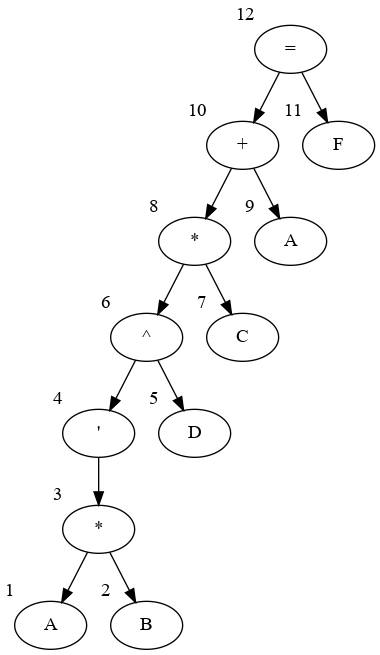
\includegraphics[height=8cm]{figures/logictree1.png}
\caption{درخت متناظر با تابع منطقی \ref{eq:logictree1}}
\label{fig:logictree1}
\end{figure}

پس از تولید این درخت، هر عملیات منطقی به شکل یک جستجوی اولویت‌دار (\itname{prioritized search}) انجام می‌شود، بدین ترتیب که برای هر رأس
\begin{enumerate}
\item
در صورتی که فرزند چپ موجود باشد، عملیات به شکل بازگشتی روی فرزند چپ
\item
در صورتی که فرزند راست موجود باشد، عملیات به شکل بازگشتی روی فرزند راست
\end{enumerate}
انجام می‌شود. به عبارت دیگر همواره فرزند چپ به فرزند راست اولویت دارد. اولویت‌بندی گره‌ها در شکل \ref{fig:logictree1} با استفاده از اعداد کنار آن‌ها مشخص شده است. 

با این وصف ابتدا \lr{assign statement} به شکل یک درخت درآمده، سپس هر عملیاتی با استفاده از یک جستجوی اولویت‌دار بر روی آن انجام می‌شود. فهرستی از توابعی که بدین منظور نوشته شده‌اند، در کد \ref{lst:assigns} آمده است. 

\lstset{caption={توابع پردازش assign statement},label=lst:assigns}
\LTR{
\begin{lstlisting}
void traverser (logicset::node* v)
void unify_operators (logicset::node* v)
void fix_assignment (logicset::node* root)
void fix_nodeid (logicset::node* node, int& cid)
void switch_childs (logicset::node* node)
void addclause (logicset::node* node, cnf_express& expression)

void prioritized_search (logicset::node* v, void(*func)(logicset::node*) = &traverser, bool after = false)
void prioritized_search (logicset::node* v, void (*func)(logicset::node*, auto&), auto& arg, bool after = false)

logicset::node* parse_assign_statement (std::string str)
cnf_express verilogexp_to_cnf_express (logicset::node* root)
\end{lstlisting}}\RTL{}

همان‌طور که مشاهده می‌شود، برای تشکیل درخت منطقی از داده‌ساختار توصیف‌شده در \codename{logicset} (قسمت \ref{section:logicset}) استفاده شده است. توابع فوق در سه دسته‌ی کلی بررسی می‌شوند.

\subsubsection{جستجوی اولویت‌دار}
\idxfunc{prioritized\_search}
تابع \codename{prioritized_search} برای جستجوی اولویت‌دار تعریف شده و یک تابع را به عنوان آرگومان ورودی می‌گیرد و آن برای تمام رأس‌های درختی که ریشه‌اش به عنوان ورودی داده شده، اجرا می‌کند. با استفاده از پارامتر \codename{after} می‌توان مشخص کرد که تابع هنگام ورود به رأس (\codename{false}) یا هنگام خروج از آن (\codename{true}) فراخوانی شود. همچنین می‌توان یک متغیر را به شکل reference در اختیار تابع قرار داد تا تغییرات لازم را روی محتوای آن اعمال کند. 

\subsubsection{پردازش گره‌ها}
توابع این بخش آن‌هایی هستند که به منظور استفاده در کنار \codename{prioritized_search} و اعمال‌شدن بر روی تک‌تک گره‌ها نوشته شده‌اند. 
\begin{itemize}

\item \codename{traverser} \idxfunc{traverser}
کار خاصی نمی‌کند و صرفا به عنوان الگوی تعریف توابع دیگر به کار می‌رود. 
\item \codename{unify_operators} \idxfunc{unify\_operators}
با فراخوانی \codename{unify_op_symbol} (بخش \ref{unifyopsymbol}) برای هر گره تمامی نمادهای منطقی استفاده‌شده را یکسان‌سازی می‌کند. 
\item \codename{fix_assignment} \idxfunc{fix\_assignment}
با توجه به تفاوت کارکرد عملگر assignment (=) نسبت به سایر عملگرها، این تابع به طور خاص آن را اعمال می‌کند. 
\item \codename{fix_nodeid} \idxfunc{fix\_nodeid}
از فیلد \codename{id} برای نگه‌داری نام متغیر متناظر با هر گره استفاده می‌شود. با توجه به این که روش تعیین نام گره‌های حاوی عملیات منطقی و گره‌های حاوی متغیر فرق دارد، این تابع اطمینان حاصل می‌کند که همه‌ی گره‌ها به درستی نام‌گذاری شده‌اند. 
\item \codename{switch_childs} \idxfunc{switch\_childs}
فرزند سمت چپ و فرزند سمت راست را جابه‌جا می‌کند. برای تصحیح اولویت عملیات منطقی کاربرد دارد. 
\item \codename{addclause} \idxfunc{addclause}
جمله‌های متناظر با گره را تولید کرده و به نمایش cnf express تابع اضافه می‌کند. 
\end{itemize}

\subsubsection{توابع سطح بالا}

دو تابع \codename{parse_assign_statement} و \codename{verilogexp_to_cnf_express} به عنوان رابط سطح بالا جهت فراخوانی از خارج کتابخانه نوشته شده‌اند. 
\begin{itemize}
\item \codename{parse_assign_statement}: \idxfunc{parse\_assign\_statement}
یک رشته حاوی یک assign statement (منهای \codename{assign}) را گرفته، درخت متناظر آن را تولید می‌کند و اشاره‌گری به ریشه‌ی آن را برمی‌گرداند. 
\item \codename{verilogexp_to_cnf_express}: \idxfunc{verilogexp\_to\_cnf\_express}
درخت تولیدشده توسط تابع فوق را ورودی گرفته، با پیمایش گره‌های آن نمایش cnf express معادل را تولید کرده و برمی‌گرداند. 
\end{itemize}

\lr{%\begin{multicols}{2}
\printindex
%\end{multicols}
}

\end{document}
